%% Template for SDP report, adapted from mlp_cw2_template, 2018. 

%% Based on  LaTeX template for ICML 2017 - example_paper.tex at 
%%  https://2017.icml.cc/Conferences/2017/StyleAuthorInstructions

\documentclass{article}
\usepackage[T1]{fontenc}
\usepackage{amssymb,amsmath}
\usepackage{txfonts}
\usepackage{microtype}
\usepackage{xspace}
\xspaceaddexceptions{\%}

% Lists with less spacing between items
\usepackage{paralist}

% For figures
\usepackage{graphicx}
\usepackage{subfig} 

% For citations
\usepackage{natbib}

% For algorithms
\usepackage{algorithm}
\usepackage{algorithmic}

% the hyperref package is used to produce hyperlinks in the
% resulting PDF.  If this breaks your system, please commend out the
% following usepackage line and replace \usepackage{mlp2017} with
% \usepackage[nohyperref]{mlp2017} below.
\usepackage{hyperref}
\usepackage{url}
\urlstyle{same}

% Packages hyperref and algorithmic misbehave sometimes.  We can fix
% this with the following command.
\newcommand{\theHalgorithm}{\arabic{algorithm}}


% Set up MLP coursework style (based on ICML style)
\usepackage{mlp2018}
\mlptitlerunning{SDP Demo \demoNumber  Group (\groupNumber)}
\bibliographystyle{icml2017}


\DeclareMathOperator{\softmax}{softmax}
\DeclareMathOperator{\sigmoid}{sigmoid}
\DeclareMathOperator{\sgn}{sgn}
\DeclareMathOperator{\relu}{relu}
\DeclareMathOperator{\lrelu}{lrelu}
\DeclareMathOperator{\elu}{elu}
\DeclareMathOperator{\selu}{selu}
\DeclareMathOperator{\maxout}{maxout}







%% You probably do not need to change anything above this comment

%% REPLACE the details in the following commands with your details
\setGroupNumber{18}
\setGroupName{Opticane}
\setProductName{Opticane}
\setDemoNumber{3}
\setLogoFileName{figs/opticane-logo.png}

\begin{document} 

\makeSDPTitle{Demo}

% Previous MLP Style Title Layout working. 
% \twocolumn[
    % \mlptitle{\productName: SDP Demo \demoNumber}
    % \centerline{Group \groupNumber: \groupName}
% ]

\begin{abstract} 
Opticane is a self-contained cane for the visually impaired that translates a user's surroundings to haptic feedback in the handle.

For the third demo, we've made significant progress in software, hardware, 3D modeling, and background research. We've integrated our purchased hardware components, worked on experimental and technically challenging features, started on our website, and finalized our 3D model for 3D printing, conducted literature review, conducted an ethics review, and finalized our interview process.
\end{abstract} 

\section{Project plan update} 

After receiving our last demo's feedback and receiving ethics research consent forms, the goals that we planned to achieve for this demo were:
\begin{itemize}
    \item Hardware 3.1: Attach stationary LIDAR to servo motor and get directional readings (achieved)
    \item Hardware 3.2: Control 5 disc vibration motors (achieved)
    \item Software 3.1: Implement simple offline speech recognition (achieved)
    \item Software 3.2: Implement simple facial recognition (achieved)
    \item Software 3.3: Implement simple haptic navigation (achieved)
    \item Software 3.4: Implement website template (achieved)
    \item Design 3.1: 3D model LIDAR casing (achieved)
    \item Design 3.2: 3D mode Opticane's interior (achieved)
    \item Research 3.1: Conduct quantitative tests (achieved)
    \item Research 3.2: Finalize usability interview questions (achieved)
    \item Research 3.3: Write ethics report (achieved)
    \item Research 3.4: Continue literature review (achieved)
\end{itemize}

Our group was able to achieve all of these goals and in doing so, increase our technical difficulty as well as prepare for prototyping. To meet these goals, we utilized Trello, Github, and Microsoft Teams with detailed tickets, thoroughly reviewed code pull requests, and weekly scrum meetings.

To promote parallel working, we split our group into teams similarly to the last demo. This time, Yuanting and Lewis worked on hardware; Samuel, Wazeed, and Austin worked on software; Shaoqing and Ioana worked on design; and Iman worked on research with help from Lewis and Ioana.

Working on these separate parts, we estimate that we've spent about 195 hours total on demo 3. Compared to demo 2, in demo 3, we've focused a lot more time on increasing technical complexity and less time on 3D modeling which we plan on finalizing and printing for the final demo. In addition, in this demo, we've tried to come up with more numerical results for quantitative analysis. The task breakdown is covered in figure \ref{fig:tickets}.

\begin{figure}[tb]
\vskip 5mm
\begin{center}
\centerline{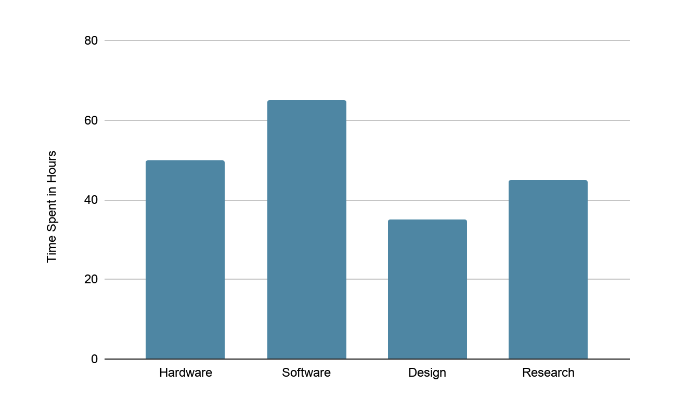
\includegraphics[width=\columnwidth]{figs/time-breakdown}}
\caption{Time Breakdown}
\label{fig:time-fig}
\end{center}
\vskip -5mm
\end{figure} 

Moving forward, For our final demo, we want to focus on completing our user guide, completing and polishing our website, and constructing a working prototype of Opticane. With these new focuses, we expect to have a complete and working prototype in-person, website, and user guide for demo 4.

\section{Technical details}

\subsection{LIDAR}

To start, in terms of hardware, we've focused our efforts on utilizing ordered parts for a prototype. Lewis has been working with the Benewake TF Luna LIDAR, a stationary, small, and lightweight LIDAR. The caveat of the LIDAR, however, is that it is stationary and so in order to accurately receive directional distance measurements, we have to attach it to a servo motor which is fortunately available in Appleton in various sizes.

Previously, we used the Turtlebots' mounted LDS-01 spinning LIDAR to aid the demonstration fo our proof of concept. This LIDAR and similar spinning ones, however, are quite expensive and heavy; the LDS-01 costs £179.90 and weighs 450 grams while the TF Luna costs £15.24 and weighs 5 grams. Comparing the two approaches, while using a stationary LIDAR and servo motor requires more work to set up, the combination offers us a much cheaper and lighter alternative to commercially affordable spinning LIDARs.

Continuing from our last demo, the method that we used to interpret the LIDAR data was to take the 180° of measurements and split it into 5 partitions. From there, we take the minima of weighted averages across every three adjacent degrees of measurement in each partition to try to decrease the impact of any noise on the LIDAR measurements.

The challenges of tackling this have mainly been on setting up the hardware of the LIDAR. The first few days that we tried to work with the LIDAR ended up not being very productive because it turned out that the LIDAR required a specific wire to interface with our raspberry pi and we needed the assistance of the technician team in both finding and solving that problem which spanned multiple days. After that, another problem we ran into was the hard to interpret documentation of the LIDAR product coupled on top of the fact that no one in the group had any raspberry pi experience.

\subsection{Haptic Feedback}

From our last demo, we used lightbulbs as a proof of concept of Opticane's functionality to demonstrate the varying intensities of haptic feedback through lightbulb intensity responding to different distance measurements from the LIDAR. Since then, Yuanting has been working on translating that feedback to our ordered mini disc vibration motors. We chose to use vibration as feedback instead of sound because sounds are less reliable in loud scenarios. The vibration motors that we use also are cheap and lightweight, costing £0.92 and weighting less than 1 gram each. They can also be vibrated in different patterns to communicate different messages.

To work with the vibration motors, we first connected one motor to the raspberry pi using an i2c connection. After we were able to work with a single motor, we found that we needed the technician team to use a multiplexer to allow for multiple i2c connects for our 5 vibration motors.

\subsection{Speech Recognition}

To increase our technical difficulty, we've decided to integrate speech recognition into our project. On the press of a button, Opticane listens to the user for a voice-activated command. Samuel has been working on getting an offline speech recognizer to register different commands. Currently, these commands are related to haptic navigation and facial recognition.

Using CMU Sphinx as our offline speech recognizer, we listen to the user's audio through a microphone until there is a pause and then work off of that audio sample. We then look at the beginning of the audio to look for command phrases such as "save location", "where is", "remember face", or "check battery".

We've set the groundworks for these commands but haven't connected all of the functionalities yet. "Save location [location-name]" saves the user's current longitude and latitude as a marker which can then be navigated towards in the future using "where is [location-name]. Similarly, "remember face [person-name]" will save the faces in front of the user which will then be recognized in the future when Opticane gets close to an object and recognizes a familiar face. "Check battery" would communicate the battery life of Opticane through haptic feedback.

We considered using Google Speech Recognition, Wit.ai, Microsoft Bing Voice Recognition, Houndify API, IBM Speech to Text, and Snowboy Hotword Detection for speech recognition as well, but while they perform better than CMU Sphinx, almost all of them require an internet connection to work. Snowboy Hotword Detection is also offline, but it stopped developer support in December of 2020 so wouldn't be extensible.

Challenges that we faced in setting up speech recognition are mainly related to the installation of CMU Sphinx which was quite convoluted for different operating systems and required a lot of other dependencies.

\subsection{Haptic Navigation}

Another feature that we are exploring is the use of our haptic feedback for performing simple navigation. Austin has been working on a script where given the user's location, the direction the user is heading in, and the destination, we use haptic feedback to indicate the direction towards the destination relative to the user. This method requires a raspberry pi GPS unit which can read Opticane's longitude, latitude, and heading, where the heading is the direction that the GPS is moving in degrees with 0° being magnetic north.

The haptic feedback that the navigation translates to is a simple vibration of some of the 5 motors that corresponds to the directional partition that the destination lies in. When the destination is behind the user, the motor corresponding to the front partition is vibrated as well and when the destination is direction behind the user, then the middle three motors are all vibrated at once. These vibrations would also be in a different pattern to the vibrations that signal object detection.

Similar to speech recognition, we attempt to combat ethical concerns by keeping all saved locations that could be navigated towards locally and plan to keep the raspberry pi offline.

\subsection{Facial Recognition}

In addition to both speech recognition and haptic navigation, we have also been exploring facial recognition for recognizing familiar faces. Wazeed has been working on a script that after saving some faces, we can then recognize them to notify the user that they are near a familiar face. Saving a face would be activated through voice-activation and then recognizing familiar faces would be automatically performed whenever Opticane detects that objects are close to the user.

Again, facial recognition brings into question many ethical concerns. Due to the high number of concerns such as dataset bias and consent of others of having their pictures taken and saved, we're planning on not going through with facial recognition in our final iteration of Opticane as suggested by Benedetta. Furthermore, the use of a camera may burn out our battery on top of our LIDAR's battery use which has been stressed to us by Ryan.

\subsection{3D Model}

For prototyping, Shaoqing and Ioana have been focusing on getting our 3D models 3D print ready. This includes hollowing out our 3D model, cutting holes for our vibration motors, and adding cases for our raspberry pi and battery which will be supported by beams to stay in place in the handle. We've also 3D modeled a case to hold our LIDAR and servo combination in place.

We're currently speaking with Garry planning our 3D print which will then allow him to fit our hardware components into a prototype Opticane handle. We plan on having a barebones but working prototype of Opticane in-person for demo 4. This prototype would be a grooved handle with haptic feedback through vibration motors with an attached LIDAR. The cane portion would be missing as it isn't vital for our proof of concept.

\subsection{Website}

Finally, to get ready to present our website for the March 30th deadline, Samuel has started work on our website by implementing a basic template and uploading it to the SDP Group 18 webserver.

\section{Evaluation}

\subsection{Quantitative Analysis}

To check if the Lidar can detect moving objects we tested it with objects moving at different speeds - 1.5m/s (walking), 5m/s (running), 7m/s (cycling), 30m/s (car). From our simulation, we concluded that the speed of the object does not affect the LIDAR output.

We also tested if swinging the cane at different speeds (0.5m/s, 2m/s, 3.5m/s, 5m/s) affects the LIDAR output. What we observed from our simulation was that while swinging the cane, if the object falls in a different partition then the LIDAR output will also change to that partition. 

In addition, with haptic feedback, due to the simplicity of the indication using each partition as a direction, there will be slight inaccuracies with the generality of the direction indicated through feedback. Because the partitions span 36° each, the general indicated direction will be off by about 9.50°. We are okay with this inaccuracy as the feature is only meant to indicate the general direction of the user's desired destination.

For speech recognition, through CMU Sphinx's offline recognizer, we have found that the accuracies vary for different commands. When referencing location names using "save location [location-name]" and "where is [location-name]", we have found an accuracy of about 40\% while "remember face" and "check battery" have an accuracy of about 70\%. With more time, we can improve the accuracy of the location name using acoustic models. We believe that the inaccuracy is due to the lack of usb microphone when testing which was recommended in documentation and also possibly due to English not being a native language when testing.

\subsection{Literature Review}

One of the features we are designing and intending to add to the cane is GPS support. This would be in the form of a haptic feedback guiding system that gives vibrations in certain directions to guide users towards object locations. We made the decision to add this based on the amount of literature references to the problem of navigation for blind people. Jack Loomis from University of California point this out in his paper: “The blind individual has a considerable disadvantage because they do not have access to location information.” \cite{sugiyama2019} Loomis makes the point that visually impaired people do not have the benefit of recognising landmarks, buildings etc as an indication of location and existing map technologies are not sufficient for this user-base. For example Google Maps only introduced voice-guided maps in 2019 and the voice-guiding technology only exists in certain countries and for certain languages (i.e mostly English). We felt by adding this haptic-guiding technology to our cane it would give blind users a similar sort of navigation information as sighted-users while also removing the need for language translation of navigation that audio-based navigation requires. This would also make our product more competitive with others on the market such as the WeWalk smart cane which requires the addition of a smartphone for navigation - our location information would come from an offline GPS unit in a raspberry pi. \cite{wewalk2020}
 
Speech recognition is another feature we are exploring, with plans to add to future iterations or versions of our cane. This speech recognition would be used to activate the haptic guiding system with sound input coming from a small microphone in the cane and toggled on and off by holding a button on the cane. Often for guiding systems, users would have to input data on a keyboard or app, for a blind person this introduces the complexity/issue of how usable those input devices are. Sound on the other hand is universal and by using saved location names we can narrow down the possible voice commands the system will pick up; allowing for less errors of incorrect locations given by speech which Hersh, Johnson and Keating point out as being “less reliable in noisy outdoor environments.” \cite{hershJohnsonKeating2008}
 
We have also done further research in a question posed in our last literature review: can our product replace the swinging of the cane? While we were unable to find direct academic studies showing the swinging motion to be an issue, there were many anecdotal accounts of the cane getting stuck and ‘jabbing’ people. We have since found a further study by the University of Cape Coast that talked about how pupils at a blind school were unable to manoeuvre objects as there “were numerous potholes and (obstacles) that hampered movement”. \cite{attiaBempong2020} The researchers concluded that typical indoor environments such as schools prevent the “free movement” of a white cane to detect such obstacles. This is the first study we have found which directly points to issues of swinging white canes and perhaps could justify our product as reducing the need for users to swing a white cane due to the rotating LIDAR.

\subsection{Ethics Report}

It is obvious that designing plays an important role in assistive technologies. A poorly designed interface can have a very poor impact on a certain group of people. Thus, designers and developers have a responsibility not to marginalize atypical users. The designers and developers should be morally aware of the importance of investing time in research, testing the product, including disabled people in their tests and getting properly trained to do their work. To be more inclusive, we will make customized handle designs to account for various grip methods used by individuals.

Next, we will analyze some ethical implications of AI for disabled people through the lens of fairness and justice. For example, in object recognition, "a recent paper demonstrates that systems using computer vision are developed largely in a white, western and middle-class context, failing to recognize common household objects that are more-often found in poor or non-western environments." \cite{bennettKeyes2019} These biases might risk harming already marginalized people from both wider communities and disabled communities. One other interesting thing to note is that "a computer vision system for accessibility, while rendering things more accessible, does so by shifting the center of analysis and judgment away from the user and towards the technology in hand." \cite{bennettKeyes2019} Even when computer vision is correctly implemented it legitimizes surveillance whose misuse can lead to a lot of problems. This also raises the question “how could technology to assist a blind person be kept from integration into policing technologies; who’s to say blind people aren’t among the users of policing technologies?” \cite{bennettKeyes2019}

There have also been concerns regarding the bias of facial recognition systems concerning ethnic minorities. Studies have shown that "the accuracies of face recognition systems used by US-based law enforcement are systematically lower for people labeled female, Black, or between the ages of 18—30 than for other demographic cohorts." \cite{buolamwiniGebru2018} There is "a lack of datasets labeled by ethnicity that limits the generalizability of research exploring the impact of ethnicity on gender classification accuracy." \cite{buolamwiniGebru2018} A gender classification accuracy report from the National Institute for Standards and Technology in the US showed that none of the 10 locations used in the study were in Africa or the Caribbean where there are significant Black populations. Using a facial recognition system could also represent a privacy issue as the system will be taking a photo of nearby individuals which would require their consent. Because of these concerns, we have decided to not move forward with computer vision and facial recognition for production.

\section{Budget}

In terms of budget, for demo 3, we haven't made any additional purchases for components. Currently as it stands, with all of our parts, the combination of LIDAR, vibration motors, rechargeable battery, servo motor, multiplexer, 3D print, and raspberry pi sum up to cost about £65. An additional GPS unit, light sensor, button, and microphone will cost about £30.

We also met with Benedetta to discuss ethical concerns of Opticane as well as to review our interview process and Christopher to discuss methods of performing quantitative analysis on our product because it is so hardware focused leading to complications with COVID-19 because most of our testing would be in-person testing and user testing. We also tried to meet with Ryan again, but due to time zone differences, we missed a last minute confirmation on a meeting time.

For technician time, our group has spent a significant amount of time working with hardware. This is largely due to our progress being bottlenecked by the fact that we can't actually physically work with the hardware and we have to go through Garry and the technician team for setting hardware up, which for the most part, doesn't work on the first attempt. While Garry and the technician team have been nothing but helpful, they still have to tend to other teams and because our project is so hardware focused for demonstrations, it was quite difficult to work at an efficient pace. One moment, a connection of the multiplexer is faulty and the next the LIDAR requires a special wire in order to work. Garry has been incredibly helpful though, even contacting us during out of work hours to try to solve problems. Taking all of this into account, we spent about 4 hours asking the technician team for help and waiting for them to get to our group and fix our wiring and other hardware issues.

\section{Video}

\href{https://uoe-my.sharepoint.com/:v:/g/personal/s1870157_ed_ac_uk/EZqwO36IaARNh3at2NdNj7MBCREfd1ZNFWt3w-I8Hk6_nA?e=5qVUbM}{video}

\begin{figure}[tb]
\vskip 5mm
\begin{center}
\centerline{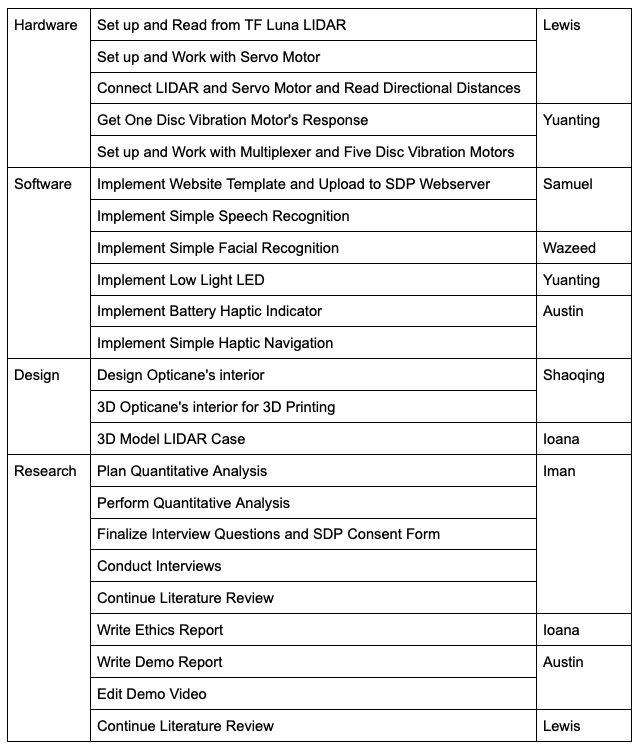
\includegraphics[width=\columnwidth]{figs/task-breakdown}}
\caption{Task Breakdown}
\label{fig:tickets}
\end{center}
\vskip -5mm
\end{figure} 

%% Include any references in a bibliography
\bibliography{example-refs}

\end{document} 

